\subsection{Multi-source Even Data Fraction}
We extend the single source assignment to multi-source assignment problem\cite{jia2010scheduling} \cite{Liu_1schedulingdivisible}.  According to each processor, we concentrate on the processors' geographical location $P_{i}$, data fraction assigned $\alpha_{i}$.
\\
Assuming the data fraction is even.  For example, the workload is unit $1$ and there are $k$ different data injection options.  So each data injection is assigned $\frac{1}{k}$ workload.
From the data injection position relationship we consider three different situations :
\begin{itemize}
\item Data injection positions consist of a subgraph $G_{L}$ of $G$.
\item Data injection processor doesn't connect with each other.
\item Other situations.
\end{itemize}

\subsubsection{Situation \uppercase\expandafter{\romannumeral1}}
If the data injection positions consist of a subgraph of $G$, we use $G_{L}$ to present it.
\begin{figure}[!ht]
\centering
\includegraphics[width=0.5\columnwidth]{figure/subgraph1.jpg}
\caption{Data injection consists of a subgraph of $G$}
\label{fig:subgraph1}
\end{figure}

\begin{figure}[!ht]
\centering
\includegraphics[width=0.5\columnwidth]{figure/subgraph2.jpg}
\caption{Data injection consists of a subgraph of $G$}
\label{fig:subgraph2}
\end{figure}
\newpage

\Fig{subgraph1} and \Fig{subgraph2} illustrate two examples that the data injections consist of subgraph $G_{L}$ of $G$. 
\newpage 
Our objective is to propose a general algorithm framework to tackle this situation and give quantity model analysis.   This algorithm is named as \textbf{\textit{Two Phase Scheduling Algorithm (TPSA)}}.

\begin{algorithm}
\caption{Two Phase Scheduling Algorithm (TPSA)}
\begin{algorithmic} 

\floatname{algorithm}{Procedure}
\renewcommand{\algorithmicrequire}{\textbf{Input: $n$ data injection positions}}
\renewcommand{\algorithmicensure}{\textbf{Output: $m*n$ processor data fractions}}
\STATE $global_{s}$ : 
\STATE Collapse the data injection processors into one ``big" equivalent processor\cite{robertazzi1993processor}.
\STATE Calculate $m*n$ processor's $D_{i}$
\STATE Obtain the flow matrix $A_{i}$.
\STATE Calculate $m*n$ processors data fraction $\alpha_{i}$
\STATE $local_{s}$ :  
\STATE Re-distributing workload between the data injection processors.
\end{algorithmic}
\end{algorithm}

\begin{itemize}
\item The time complexity is $O(k*m*n)$.
\item The time to calculate each determinant is $O(n^{3})$ with Gaussian elimination or LU decomposition.  So the total determinant time complexity is $O(k*n^{3})$.
\item The total time complexity is $O(k*n^{3})$.  Nonetheless, in real case, the time complexity is fast enough.  
\end{itemize}

\newpage


For example, \Fig{subgraph1}'s \textbf{\textit{flow matrix}} is :

\begin{equation}
{
\left[ \begin{array}{cccccc}
4 & 8 & 12 & 10 & 6 & 2\\
1 & -1 & 0 & 0 & 0 & 0\\
0 & \sigma-1 & 1 & 0 & 0 & 0\\
0 & \sigma-1 & \sigma & 1 & 0 & 0\\
0 & \sigma-1 & \sigma & \sigma & 1 & 0\\
0 & \sigma-1 & \sigma & \sigma & \sigma & 1\\
\end{array} 
\right ]} \times \left[ \begin{array}{c}
\alpha_{0} \\
\alpha_{1} \\
\alpha_{2} \\
\alpha_{3} \\
\alpha_{4} \\
\alpha_{5}
\end{array} 
\right ] = \left[ \begin{array}{c}
1 \\
0 \\
0 \\
0 \\
0 \\
0
\end{array} 
\right ]
\end{equation}
The simulation result illustrates as follows:

\begin{figure}[!ht]
\centering
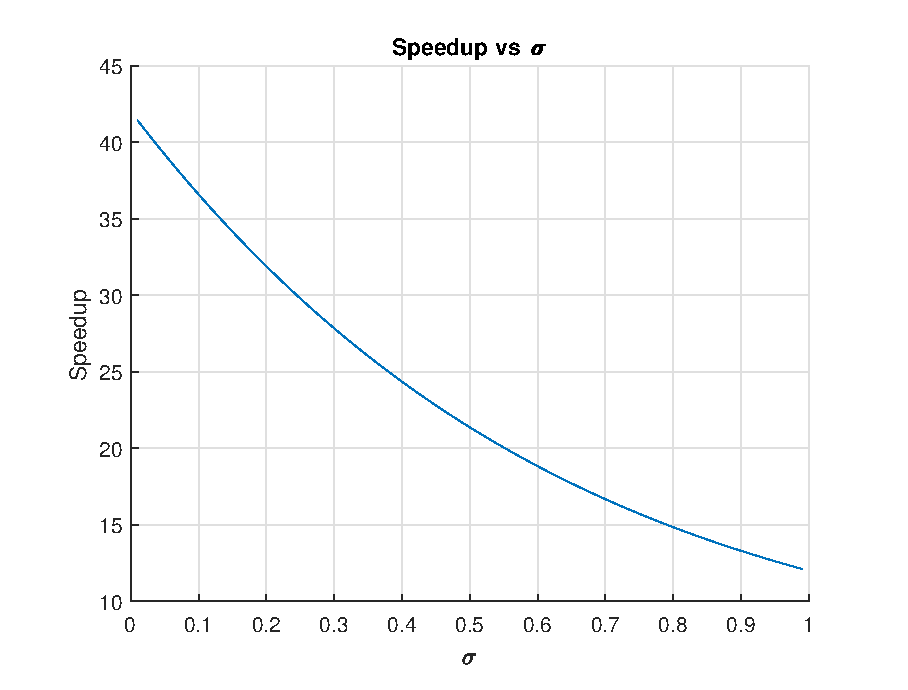
\includegraphics[width=1\columnwidth]{figure/vo_sub1.eps}
\caption{Speedup vs $\sigma$}
\label{fig:vo_sub1}
\end{figure}

\begin{figure}[!ht]
\centering
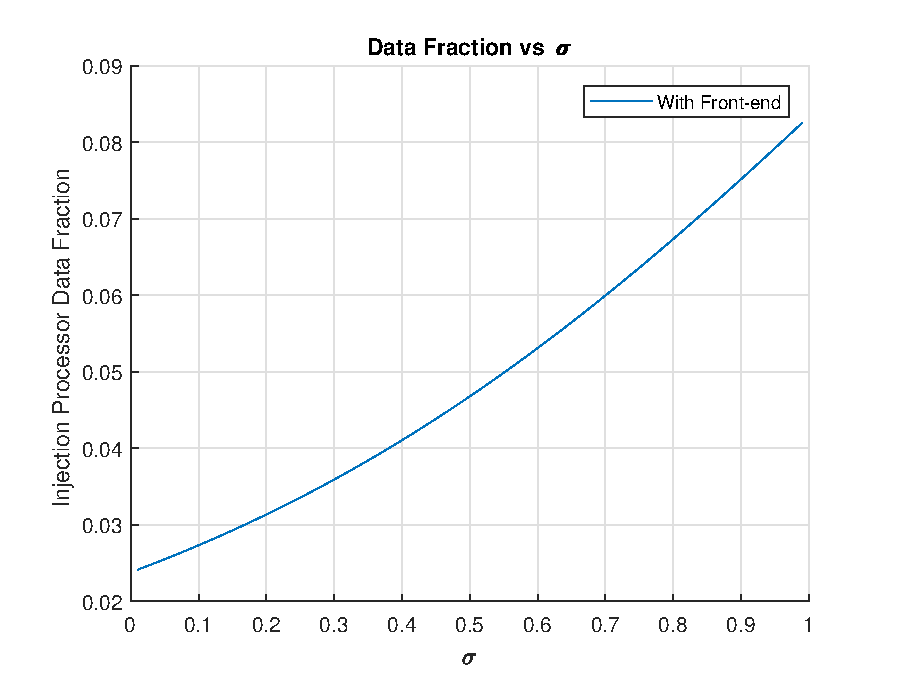
\includegraphics[width=1\columnwidth]{figure/vo_sub1_fraction.eps}
\caption{Injection Processor Data Fraction vs $\sigma$}
\label{fig:vo_sub1_fraction}
\end{figure}

This simulation says the best performance happens on value $\sigma \leq 0.05$, which hits about $40$ times speedup.  If $\sigma \approx 1$, the network achieves almost $12$ times performance.  In addition, the data fraction in each injection processors are the same, that is, there is no need to transfer data between local processors.
\newpage

For example, \Fig{subgraph2}'s \textbf{\textit{flow matrix}} is :

\begin{equation}
{
\left[ \begin{array}{ccccccc}
7 & 14 & 15 & 10 & 6 & 3 & 1\\
1 & -1 & 0 & 0 & 0 & 0 & 0\\
0 & \sigma-1 & 1 & 0 & 0 & 0 & 0\\
0 & \sigma-1 & \sigma & 1 & 0 & 0 & 0\\
0 & \sigma-1 & \sigma & \sigma & 1 & 0 & 0\\
0 & \sigma-1 & \sigma & \sigma & \sigma & 1& 0\\
0 & \sigma-1 & \sigma & \sigma & \sigma & \sigma & 1\\
\end{array} 
\right ]} \times \left[ \begin{array}{c}
\alpha_{0} \\
\alpha_{1} \\
\alpha_{2} \\
\alpha_{3} \\
\alpha_{4} \\
\alpha_{5}
\end{array} 
\right ] = \left[ \begin{array}{c}
1 \\
0 \\
0 \\
0 \\
0 \\
0
\end{array} 
\right ]
\end{equation}
The simulation result illustrates as follows:

\begin{figure}[!ht]
\centering
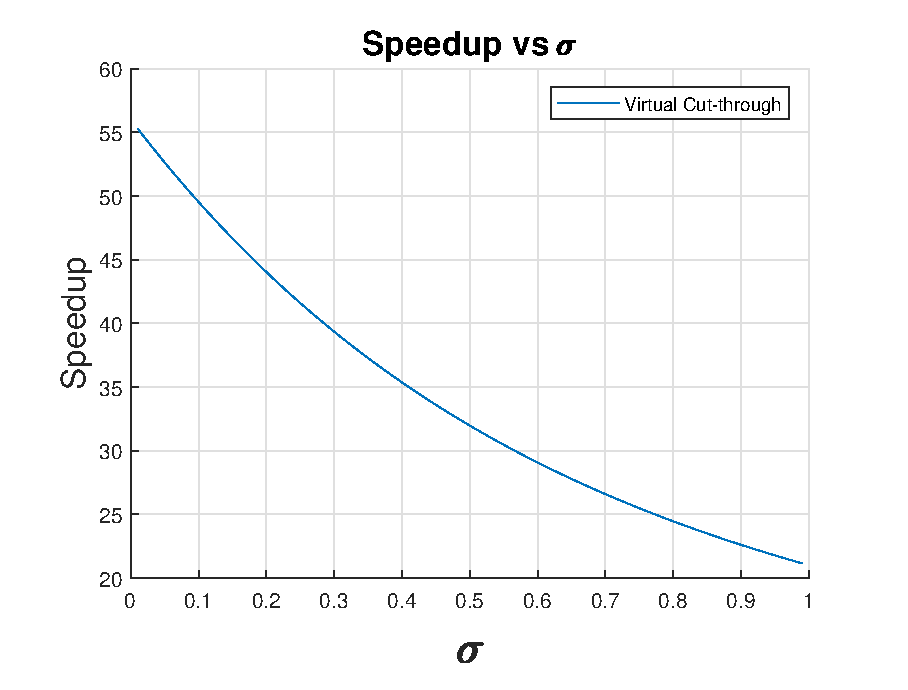
\includegraphics[width=1\columnwidth]{figure/vo_sub2.eps}
\caption{Speedup vs $\sigma$}
\label{fig:vo_sub2}
\end{figure}

\begin{figure}[!ht]
\centering
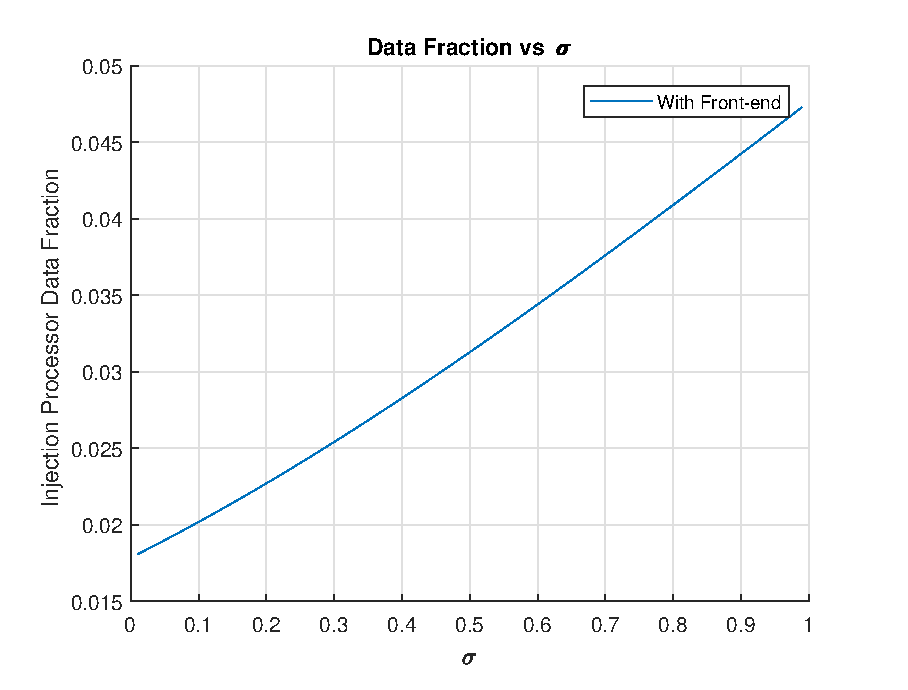
\includegraphics[width=1\columnwidth]{figure/vo_sub2_fraction.eps}
\caption{Injection Processor Data Fraction vs $\sigma$}
\label{fig:vo_sub2_fraction}
\end{figure}

This simulation says the best performance happens on value $\sigma \leq 0.05$, which hits about $55$ times speedup.  If $\sigma \approx 1$, the network achieves almost $21$ times performance.  In addition, the data fraction in each injection processors are the same, that is, there is no need to transfer data between local processors.
\newpage

\subsubsection{Situation \uppercase\expandafter{\romannumeral2}}
The data injections don't consist of a subgraph of $G$.  
Jia \cite{fortune1995voronoi} proposes an algorithm to utilize the nearest data injection principle to tackle this scenario.  In the dividable load intricate applications, for example, big file transmission, HPC scientific computation, like BlueGene \cite{krevat2002job} or Hadoop job, the total finish time depends on the last piece ending time-stamp.  \\
Our objective is to propose a general algorithm framework to utilize less processors and achieve the same finish time.  \\

\Fig{voronoi_even_cells} shows $10$ Voronoi cells division and \Fig{voronoi_even_speedup} figures out the speedup of each cells.\\
\begin{figure}[!ht]
\centering
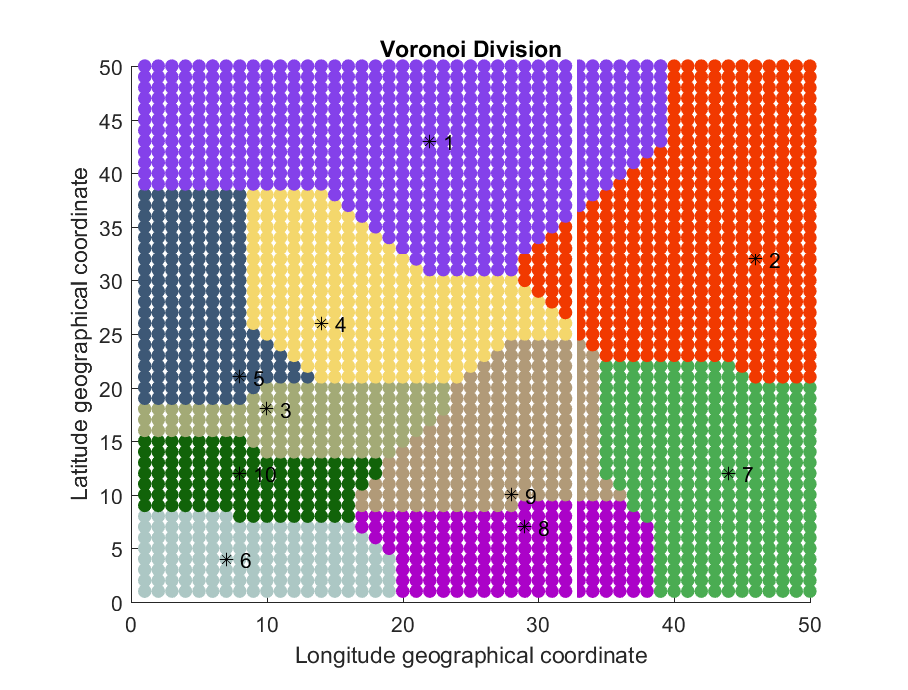
\includegraphics[width=1\columnwidth]{figure/voronoi_even_cells.eps}
\caption{$10$ Voronoi Cells}
\label{fig:voronoi_even_cells}
\end{figure}
\newpage 

\begin{figure}[!ht]
\centering
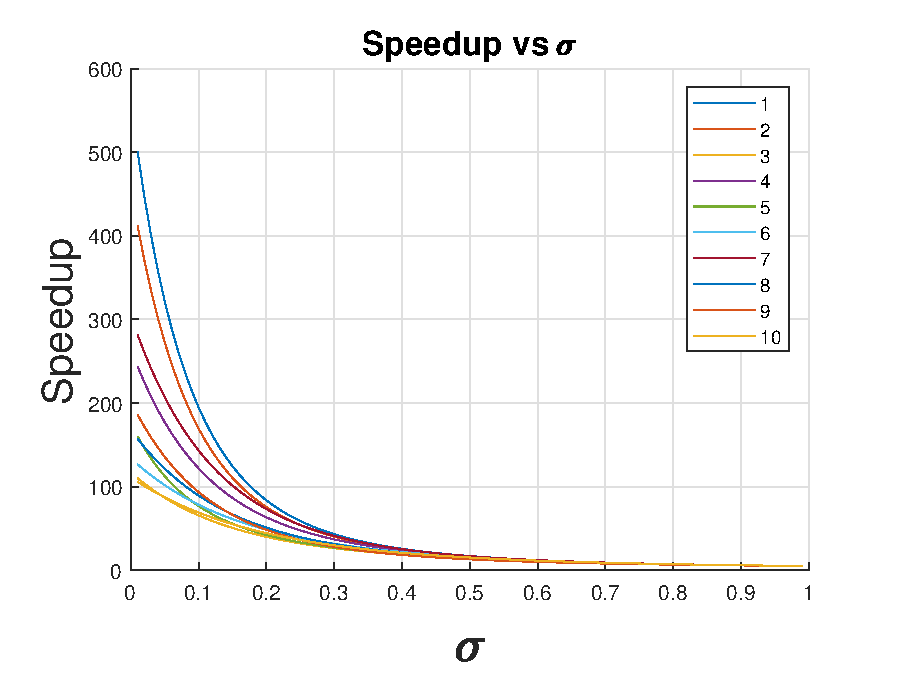
\includegraphics[width=1\columnwidth]{figure/voronoi_even_speedup.eps}
\caption{$10$ Voronoi Cells speedup curves}
\label{fig:voronoi_even_speedup}
\end{figure}

\newpage 

The heuristic algorithm is named as \textbf{\textit{Reduced Voronoi Diagram Algorithm}}:

\begin{algorithm}
\caption{Reduced Voronoi Diagram Algorithm(RVDA)}
\begin{algorithmic} 

\floatname{algorithm}{Procedure}
\renewcommand{\algorithmicrequire}{\textbf{Input: $k$ data injection position}}
\renewcommand{\algorithmicensure}{\textbf{Output: $k$ reduced Voronoi cells and $m*n$ processor data fractions}}
\STATE $global_{s}$ :
\STATE Define the cell's flow matrix column's number is $depth$.
\STATE Calculate $k$ Voronoi cells with Manhattan distance.
\STATE Calculate $k$ radius $R_{i}$ of $n$ Voronoi cells.
\STATE Calculate each cell's flow matrix $A_{i}$.
\STATE Set $depth_{min} = \min {Speedup_{i}}$'s $R_{i}$.
\WHILE{$1 \leq i \leq k$}
\STATE $tempdepth_{i} = R_{i}$

\WHILE{$ depth_{min} \leq j \leq tempdepth_{i}$}
\STATE Binary Search the  value $\min (j)$, the flow matrix $\hat{A_{i}}$'s speedup $ > \min(speedup_{min})$. 
\STATE j = j + 1.
\ENDWHILE

\STATE Calculate the Reduced Voronoi cells by setting the $depth_{i} = depth_{min}$ in each cell.

\STATE Calculate Voronoi cell's flow matrix $A_{i}$.
\STATE $ i = i + 1$
\ENDWHILE
\STATE $local_{s}$ :
\STATE Display each reduced Voronoi cells.
\STATE Illustrate each reduced Voronoi cells' speedup curves
\end{algorithmic}
\end{algorithm}
\newpage

\begin{itemize}
\item The Manhattan Voronoi cells' time complexity is $O(k*m*n)$;
\item The binary search find the $\min j$'s time complexity is $O(k*(\log_2 \max(m,n)))$.
\item So the total time complexity is $O(k*m*n)$.
\end{itemize}


\Fig{voronoi_even_cells_save} and \Fig{voronoi_even_speedup_save} show the algorithm's result and speedup curves.  The algorithm obtains the same running time yet saves about $30\%$ processors.

\begin{figure}[!ht]
\centering
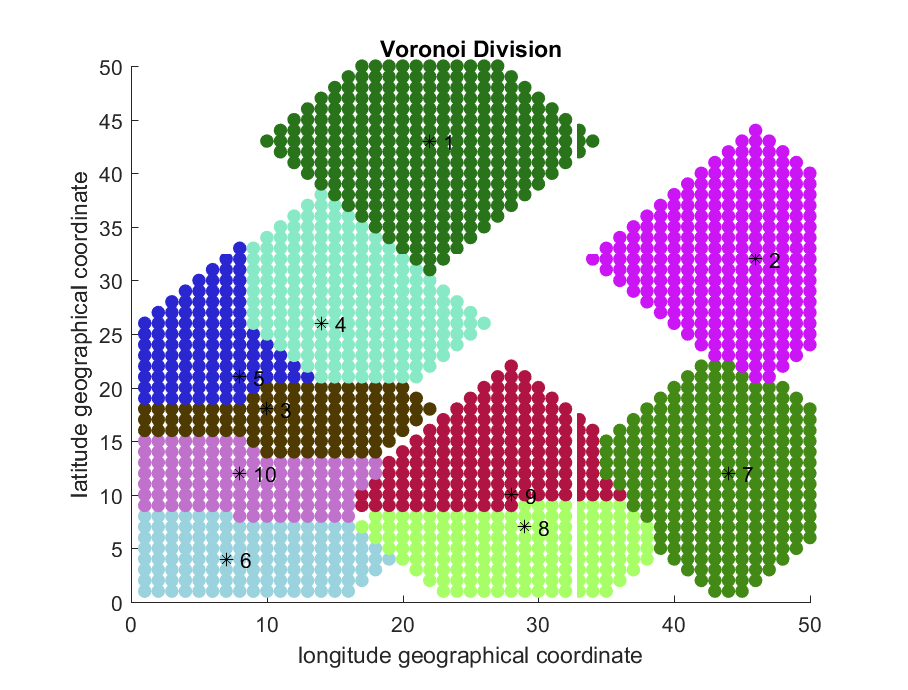
\includegraphics[width=1\columnwidth]{figure/voronoi_even_cells_save.eps}
\caption{$10$ reduced Voronoi cells}
\label{fig:voronoi_even_cells_save}
\end{figure}

\begin{figure}[!ht]
\centering
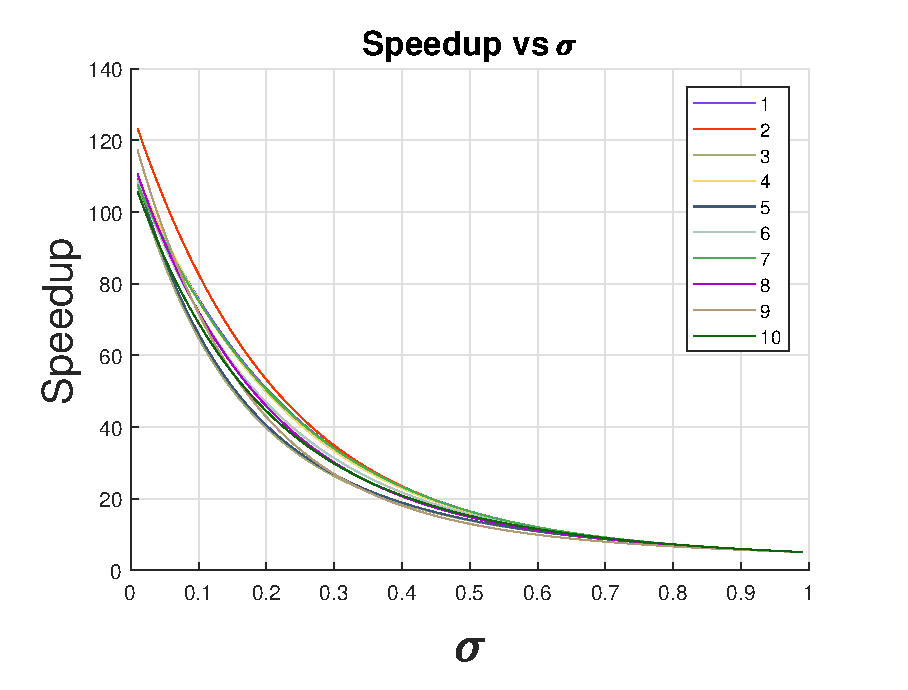
\includegraphics[width=1\columnwidth]{figure/voronoi_even_speedup_save.eps}
\caption{$10$ reduced Voronoi cells's speedup curves}
\label{fig:voronoi_even_speedup_save}
\end{figure}

\Fig{voronoi_even_speedup} shows $\sigma < 0.2$, the ratio $\max(\frac{max speedup}{min speedup}) = \frac{500}{100} = 5$ and \Fig{voronoi_even_speedup_save} shows the ratio is $\max(\frac{max speedup}{min speedup}) = \frac{270}{100} = 2.7$.  \\
It displays that $10$ pieces of processor cluster's equal computation is more balanced than initial setting, and the whole cluster finishes tasks with the same time by less processors.
\newpage
After $1000$ round random sampling experiments, we obtain the average saved processors ratio in \Fig{voronoi_save}.
\begin{figure}[!ht]
\centering
\includegraphics[width=1\columnwidth]{figure/voronoi_save.eps}
\caption{Reduced Voronoi Division Algorithm average processors' percentage}
\label{fig:voronoi_save}
\end{figure}
From \Fig{voronoi_save}, it shows the average percentage of saved processor is about $35 \%$.  
\newpage
\subsubsection{Situation \uppercase\expandafter{\romannumeral3}}
If there are some nodes consisting a subgraph and there are some nodes individual, our objective to finish the whole project in the same time and save processors and give a quantity analysis model to this data injection situation.

We process an improved RVDA algorithm to tackle this situation. 

\begin{algorithm}
\caption{Improved Reduced Voronoi Diagram Algorithm(IRVDA)}
\begin{algorithmic} 
\floatname{algorithm}{Procedure}
\renewcommand{\algorithmicrequire}{\textbf{Input: $n$ data injection position}}
\renewcommand{\algorithmicensure}{\textbf{Output: $n$ reduced Voronoi cells and $m*n$ processor data fractions}}
\STATE $global_{s}$ :
\STATE Define the cell's flow matrix column's number is $depth$.
\STATE Collapse the data injection processors into one ``big" equivalent processor.
\STATE Calculate $k$ constrained Voronoi cells\cite{chin1998finding} with Manhattan distance and get $k$ cells.
\STATE Calculate $k$ radius $R_{i}$ of $k$ Voronoi cells.
\WHILE{$1 \leq i \leq k$}
\STATE Calculate the speedup $Speedup_{i}$ with flow matrix $A_{i}$.
\STATE $ i = i + 1$
\ENDWHILE
\STATE Set the $depth_{min} = \min(Speedup_{i})$'s Radius
\WHILE{$1 \leq i \leq n$}
\STATE $tempdepth_{i} = R_{i}$.
\WHILE{$ depth_{min} \leq j \leq tempdepth_{i}$}
\STATE Binary Search the  value $\min (j)$, the flow matrix $\hat{A_{i}}$'s speedup $ > \min(Speedup_{min})$. 
\STATE  break.
\STATE j = j + 1.
\ENDWHILE
\STATE Calculate Voronoi cell's flow matrix $\hat{A_{i}}$.
\STATE $ i = i + 1$
\ENDWHILE
\STATE $local_{s}$ :
\STATE Display each reduced Voronoi cells.
\STATE Illustrate each reduced Voronoi cells' speedup curves
\end{algorithmic}
\end{algorithm}




